\documentclass[12pt,a4paper]{article}

\usepackage{fontspec}
\defaultfontfeatures{Ligatures=TeX}
\usepackage{polyglossia}
\setdefaultlanguage{russian}
\setotherlanguage{english}
\setmainfont{Times New Roman}
\setsansfont{Arial}
\setmonofont{Courier New}
\newfontfamily\cyrillicfont{Times New Roman}
\newfontfamily\cyrillicfontsf{Arial}
\newfontfamily\cyrillicfonttt{Courier New}
\usepackage{amsmath,amssymb,amsfonts}
\usepackage{amsthm}
\usepackage[margin=2.5cm]{geometry}
\usepackage[numbers,sort&compress]{natbib}
\usepackage{hyperref}
\usepackage{xcolor}
\usepackage{booktabs}
\usepackage{mathtools}
\usepackage[shortlabels]{enumitem}
\usepackage{graphicx}
\usepackage{doi}
\usepackage{tikz}
\usetikzlibrary{arrows.meta,positioning,calc,decorations.pathreplacing}

\newtheorem{theorem}{Теорема}[section]
\newtheorem{lemma}[theorem]{Лемма}
\newtheorem{corollary}[theorem]{Следствие}
\newtheorem{proposition}[theorem]{Утверждение}
\theoremstyle{definition}
\newtheorem{definition}[theorem]{Определение}
\theoremstyle{remark}
\newtheorem{remark}[theorem]{Замечание}

%%% Custom commands
\newcommand{\Weylsq}{C_{\mu\nu\rho\sigma}C^{\mu\nu\rho\sigma}}
\newcommand{\dd}{\mathrm{d}}
\newcommand{\Tr}{\operatorname{Tr}}
\newcommand{\tr}{\operatorname{tr}}
\newcommand{\half}{\tfrac{1}{2}}
\newcommand{\Lam}{\Lambda}
\newcommand{\order}{\mathcal{O}}
\newcommand{\Hilb}{\mathcal{H}}
\newcommand{\Alg}{\mathcal{A}}
\newcommand{\Dslash}{D\!\!\!\!/\,}

\hypersetup{
  colorlinks=true,
  linkcolor=blue!60!black,
  citecolor=blue!60!black,
  urlcolor=blue!60!black,
  pdfauthor={Давид Алфёров},
  pdftitle={Пертурбативная ультрафиолетовая конечность спектрального действия в D²-квантовании: доказательство киральности},
  pdfsubject={hep-th}
}

\begin{document}

\title{Пертурбативная ультрафиолетовая конечность спектрального действия\\
в $D^2$-квантовании: доказательство киральности}

\author{Давид Алфёров}

\date{Март 2026}

\maketitle

% ============================================================
\begin{abstract}
% ============================================================

Мы доказываем, что в $D^2$-квантовании спектрального действия
$S = \Tr\,f(D^2/\Lam^2)$ все пертурбативные контрчлены на каждом
петлевом порядке коммутируют с оператором киральности~$\gamma_5$ и,
следовательно, поглощаемы деформацией спектральной функции~$f$.
Доказательство является чисто алгебраическим: дираковское соотношение
киральности $\{D, \gamma_5\} = 0$ приводит к тому, что вариация
$\delta(D^2)$ коммутирует с~$\gamma_5$, и эта блочно-диагональная
структура распространяется на кинетический оператор, пропагатор,
вершины и все петлевые интегралы.  Результат устраняет трёхпетлевое
препятствие переопределённости метрического квантования, при котором два
независимых квартичных вейлевских инварианта не могут быть поглощены
единственным спектральным параметром.
Ультрафиолетовая конечность выполняется через два петлевых порядка
(где единственная структура контрчлена размерности~6 гарантирует
поглощение) и на всех пертурбативных порядках при пяти аксиомах БВ,
сформулированных в разделе~\ref{sec:gap}, --- из которых две доказаны,
одна естественна и две верифицированы на однопетлевом уровне.
Тождество проверено численно для конечных спектральных троек
($N = 4$--$64$, $L = 1$--$8$) и формально в Lean~4.  Замкнутость
является пертурбативной; непертурбативная эквивалентность остаётся
открытой.

\end{abstract}

\tableofcontents
\newpage

% ============================================================
\section{Введение}
\label{sec:intro}
% ============================================================

Пертурбативное квантование общей теории относительности приводит к
ультрафиолетовым расходимостям, которые не могут быть устранены
процедурой перенормировки.
На однопетлевом уровне чистая гравитация конечна на массовой
оболочке~\cite{tHooftVeltman:1974}, однако добавление материи или
включение двухпетлевых диаграмм вводит расходящиеся контрчлены,
пропорциональные кубу тензора
Римана~\cite{Goroff:1985th, vandeVen:1992gw}.  Расширения с высшими
производными, такие как теория Стелле с членами, квадратичными по
тензору Вейля, и $R^2$~\cite{Stelle:1976gc}, достигают
перенормируемости ценой введения духовых степеней свободы.

Принцип спектрального действия~\cite{Chamseddine:1996zu, Chamseddine:2006ep}
предлагает геометрически естественную отправную точку: гравитационное
действие есть след функции квадрата оператора Дирака,
\begin{equation}\label{eq:spectral_action}
  S = \Tr\,f\!\left(\frac{D^2}{\Lam^2}\right),
\end{equation}
где $(\Alg, \Hilb, D)$ --- спектральная тройка~\cite{Connes:1994book,
Connes:1995cr}, а $f$ --- положительная чётная функция, служащая
спектральным обрезанием на масштабе~$\Lam$.  Асимптотическое
разложение~\eqref{eq:spectral_action} воспроизводит действие
Эйнштейна--Гильберта с космологической постоянной, поправки,
квадратичные по тензору Вейля, и $R^2$, а на почти-коммутативной
геометрии --- полный бозонный сектор Стандартной
модели~\cite{Chamseddine:2010ud, vanSuijlekom:2014pya}.

В предыдущих работах~\cite{Alfyorov:2026ff, Alfyorov:2026ss} мы
вычислили полные нелокальные однопетлевые формфакторы
$F_1(\Box/\Lam^2)$ и $F_2(\Box/\Lam^2, \xi)$ для спектральной тройки
Стандартной модели и получили феноменологию спектрального действия для
Солнечной системы.  В сопутствующей работе~\cite{Alfyorov:2026ct} мы
установили \emph{теорему о киральности} для коэффициентов
Сили--ДеВитта: следовые коэффициенты ядра теплопроводности
раскладываются как $\tr(a_{2n}) = f_n(p) + f_n(q)$ с нулевыми
перекрёстными членами $pq$, где $p$ и~$q$ обозначают самодуальный и
антисамодуальный секторы тензора Вейля.  Однако на трёхпетлевом уровне
и выше в метрическом квантовании контрчлены \emph{не} ограничены
киральностью: возникают два независимых квартичных вейлевских
инварианта, но для их поглощения доступен лишь один спектральный
параметр~$\delta\psi$.  Это трёхпетлевое препятствие было
идентифицировано как основной барьер для доказательства
ультрафиолетовой конечности на всех порядках в рамках спектрального
действия.

Настоящая работа устраняет это препятствие путём изменения переменной
квантования.  Вместо разложения функционального интеграла по
возмущениям метрики~$g_{\mu\nu}$ мы разлагаем его по возмущениям
квадрата оператора Дирака~$D^2$.  Ключевое наблюдение состоит в том,
что тождество киральности $\{D, \gamma_5\} = 0$, которое выполняется
для оператора Дирака на любом спиновом многообразии, принуждает все
возмущения $\delta(D^2)$ коммутировать с~$\gamma_5$.  Это ограничение
распространяется через всё пертурбативное разложение: кинетический
оператор, пропагатор, все вершины и, следовательно, все петлевые
интегралы сохраняют киральность.  Контрчлены на каждом петлевом порядке
блочно-диагональны в киральном базисе и поэтому могут быть поглощены
деформацией $f \to f + \delta f$ спектральной функции.

Физическая эквивалентность $D^2$-квантования и стандартного метрического
квантования (открытый вопрос~G1) рассматривается на пертурбативном
уровне: мы доказываем эквивалентность через один петлевой порядок и
формулируем точные аксиомы для эквивалентности на всех порядках.  В
частности, мы показываем, что сектор духов Фаддеева--Попова метрического
квантования сохраняет киральность в спинорном базисе, и аргументируем,
что БРСТ-когомологии обеих схем изоморфны на физическом секторе.
Непертурбативная эквивалентность остаётся открытой.  Мы обсуждаем это
подробно в разделе~\ref{sec:gap}.

\medskip
\noindent\textbf{Структура работы.}
Раздел~\ref{sec:prelim} содержит обзор спектральных троек, киральности
и спектрального действия.  В разделе~\ref{sec:chirality_identity}
доказывается центральное алгебраическое тождество
$[\delta(D^2), \gamma_5] = 0$.
Раздел~\ref{sec:uv_finiteness} содержит вывод теоремы о конечности на
всех порядках.  Раздел~\ref{sec:three_loop} объясняет разрешение
трёхпетлевого препятствия.  Раздел~\ref{sec:numerics} представляет
численную верификацию.  Раздел~\ref{sec:gap} посвящён физической
эквивалентности (открытый вопрос~G1).
Раздел~\ref{sec:related} помещает результат в контекст предыдущих
работ.  Раздел~\ref{sec:conclusions} содержит заключение.

% ============================================================
\section{Предварительные сведения}
\label{sec:prelim}
% ============================================================

\subsection{Спектральные тройки}

\emph{Вещественная спектральная тройка} $(\Alg, \Hilb, D)$ состоит из
$*$-алгебры~$\Alg$, точно представленной на гильбертовом
пространстве~$\Hilb$, и самосопряжённого оператора~$D$ (оператора
Дирака) с компактной резольвентой, удовлетворяющего аксиомам
некоммутативной геометрии~\cite{Connes:1994book, Connes:1995cr,
Connes:2008vs}.  В чётной KO-размерности существует оператор
киральности $\gamma$ (который мы обозначаем $\gamma_5$ в размерности~4),
удовлетворяющий $\gamma_5^2 = 1$, $\gamma_5 = \gamma_5^*$ и условию
градуировки:
\begin{equation}\label{eq:chirality_grading}
  \{D, \gamma_5\} = D\gamma_5 + \gamma_5 D = 0.
\end{equation}

Каноническим примером является компактное риманово спиновое
многообразие~$(M, g)$, где $\Alg = C^\infty(M)$,
$\Hilb = L^2(M, S)$ --- гильбертово пространство
$L^2$-спиноров, а $D = i\gamma^\mu\nabla_\mu^S$ --- оператор Дирака,
ассоциированный со спиновой связностью.  В четырёх измерениях
$\gamma_5 = i\gamma^0\gamma^1\gamma^2\gamma^3$ раскладывает спинорное
расслоение на левые и правые вейлевские спиноры:
$S = S_L \oplus S_R$.

\subsection{Киральность в киральном базисе}

В киральном базисе
$\gamma_5 = \operatorname{diag}(+\mathbf{1}, -\mathbf{1})$, и условие
градуировки~\eqref{eq:chirality_grading} вынуждает $D$ быть
\emph{блочно-антидиагональным}:
\begin{equation}\label{eq:D_chiral_basis}
  D = \begin{pmatrix} 0 & A \\ A^\dagger & 0 \end{pmatrix},
\end{equation}
где $A\colon S_R \to S_L$.  Квадрат оператора Дирака тогда
\emph{блочно-диагонален}:
\begin{equation}\label{eq:D2_chiral_basis}
  D^2 = \begin{pmatrix} AA^\dagger & 0 \\ 0 & A^\dagger A \end{pmatrix}.
\end{equation}
Эта блочная структура является основой всего доказательства.

\subsection{Спектральное действие и его квантование}

Спектральное действие~\eqref{eq:spectral_action} зависит от $D$ только
через $D^2$.  \emph{$D^2$-квантование} осуществляется записью
\begin{equation}\label{eq:D2_quantization}
  D = D_0 + \delta D, \qquad
  D^2 = D_0^2 + \underbrace{\{D_0, \delta D\} + (\delta D)^2}_{\delta(D^2)},
\end{equation}
где $D_0$ --- фоновый оператор Дирака, а $\delta D$ --- квантовая
флуктуация, оба удовлетворяющие условию
киральности~\eqref{eq:chirality_grading}.
Функциональный интеграл берётся по пространству допустимых возмущений
$\delta D$:
\begin{equation}\label{eq:path_integral}
  Z = \int \mathcal{D}[\delta D]\; e^{-S[D_0 + \delta D]}.
\end{equation}

Это следует противопоставить \emph{метрическому квантованию}, где
$g_{\mu\nu} = \bar{g}_{\mu\nu} + h_{\mu\nu}$ и функциональный интеграл
берётся по~$h_{\mu\nu}$.  Метрика определяет~$D$ через спиновую
связность, однако отображение $g \mapsto D$ является отображением
«многие-к-одному»: различные операторы Дирака могут иметь одну и ту же
метрику~\cite{Barrett:2015matrix}.  Пространство операторов Дирака,
удовлетворяющих аксиомам спектральной тройки, поэтому \emph{больше},
чем пространство метрик (см.\ раздел~\ref{sec:gap}).

% ============================================================
\section{Тождество киральности}
\label{sec:chirality_identity}
% ============================================================

Центральный алгебраический результат:

\begin{lemma}\label{lem:anticommute}
Пусть $D$ и $\delta D$ --- операторы на $\Hilb$, удовлетворяющие
$\{D, \gamma_5\} = 0$ и $\{\delta D, \gamma_5\} = 0$.  Тогда:
\begin{enumerate}[(i)]
  \item $[D^2, \gamma_5] = 0$,
  \item $[\{D, \delta D\}, \gamma_5] = 0$,
  \item $[(\delta D)^2, \gamma_5] = 0$.
\end{enumerate}
\end{lemma}

\begin{proof}
(i)~$[D^2, \gamma_5] = D\{D, \gamma_5\} - \{D, \gamma_5\}D = 0$.

\medskip\noindent
(ii)~Раскроем:
\begin{align}
  \gamma_5 \{D, \delta D\}
  &= \gamma_5(D\,\delta D + \delta D\, D) \nonumber \\
  &= (\gamma_5 D)\,\delta D + (\gamma_5\,\delta D)\,D \nonumber \\
  &= (-D\gamma_5)\,\delta D + (-\delta D\,\gamma_5)\, D
    \label{eq:step_anticomm}\\
  &= D(\delta D\,\gamma_5) + \delta D(D\,\gamma_5)  \nonumber \\
  &= (D\,\delta D + \delta D\, D)\gamma_5 \nonumber \\
  &= \{D, \delta D\}\,\gamma_5. \nonumber
\end{align}
В шаге~\eqref{eq:step_anticomm} мы использовали
$\gamma_5 D = -D\gamma_5$ (из $\{D, \gamma_5\} = 0$) и
$\gamma_5\,\delta D = -\delta D\,\gamma_5$
(из $\{\delta D, \gamma_5\} = 0$).  Двойная смена знака даёт
тождество.

\medskip\noindent
(iii)~Аналогично:
\begin{align}
  \gamma_5\,(\delta D)^2
  &= (\gamma_5\,\delta D)\,\delta D
  = (-\delta D\,\gamma_5)\,\delta D \nonumber \\
  &= \delta D(-\gamma_5\,\delta D)
  = \delta D\,(\delta D\,\gamma_5)
  = (\delta D)^2\,\gamma_5. \nonumber
\end{align}
\end{proof}

\begin{theorem}[Киральность $\delta(D^2)$]\label{thm:chirality_deltaD2}
Пусть $D_0$ и $\delta D$ --- самосопряжённые операторы на $\Hilb$,
удовлетворяющие $\{D_0, \gamma_5\} = 0$ и
$\{\delta D, \gamma_5\} = 0$.  Тогда
\begin{equation}\label{eq:main_identity}
  [\delta(D^2), \gamma_5] = 0, \qquad
  \delta(D^2) \coloneqq \{D_0, \delta D\} + (\delta D)^2.
\end{equation}
\end{theorem}

\begin{proof}
Непосредственно следует из леммы~\ref{lem:anticommute}(ii) и~(iii):
\begin{equation}
  [\delta(D^2), \gamma_5]
  = [\{D_0, \delta D\}, \gamma_5] + [(\delta D)^2, \gamma_5]
  = 0 + 0 = 0. \qedhere
\end{equation}
\end{proof}

\begin{corollary}[Блочно-диагональная подалгебра]\label{cor:subalgebra}
Множество операторов, коммутирующих с $\gamma_5$, образует
$*$-подалгебру.  В частности:
\begin{enumerate}[(i)]
  \item Если $[A, \gamma_5] = [B, \gamma_5] = 0$, то
        $[AB, \gamma_5] = 0$.
  \item Если $[A, \gamma_5] = 0$ и $A$ обратим, то
        $[A^{-1}, \gamma_5] = 0$.
  \item Если $[A, \gamma_5] = 0$ и $g$ --- произвольная функция,
        допускающая спектральное разложение, то $[g(A), \gamma_5] = 0$.
\end{enumerate}
\end{corollary}

\begin{proof}
(i)~$\gamma_5(AB) = (\gamma_5 A)B = (A\gamma_5)B = A(\gamma_5 B) = A(B\gamma_5) = (AB)\gamma_5$.

(ii)~$\gamma_5 = \gamma_5 AA^{-1} = A\gamma_5 A^{-1}$, откуда
$A^{-1}\gamma_5 = \gamma_5 A^{-1}$.

(iii)~Для ограниченного $A$ функция $g(A)$ является пределом
полиномов от $A$ по норме; применим~(i) итеративно и перейдём к
пределу.  Для неограниченного $A$ (такого как $D^2$ на многообразии)
результат следует из спектральной теоремы для неограниченных
самосопряжённых операторов: $g(A) = \int g(\lambda)\,dE_\lambda$, где
$E_\lambda$ --- спектральное разложение.  Поскольку
$[A, \gamma_5] = 0$ влечёт $[E_\lambda, \gamma_5] = 0$ для
всех~$\lambda$, мы получаем $[g(A), \gamma_5] = 0$ посредством
функционального исчисления.
\end{proof}

\begin{remark}
Доказательство теоремы~\ref{thm:chirality_deltaD2} является чисто
алгебраическим.  Оно использует лишь соотношение антикоммутации
$\{D, \gamma_5\} = 0$ и справедливо в любой ассоциативной алгебре с
инволюцией.  В частности, оно выполняется для конечномерных матриц
(конечные спектральные тройки), для дифференциальных операторов на
многообразиях и для любого спектрального усечения в смысле
Конна--ван~Сёйлекома~\cite{Connes:2020trunc}.  Никакие приближения или
предельные процедуры не используются.
\end{remark}

% ============================================================
\section{Ультрафиолетовая конечность на всех петлевых порядках}
\label{sec:uv_finiteness}
% ============================================================

\subsection{Кинетический оператор и пропагатор}

В $D^2$-квантовании квадратичное разложение спектрального
действия~\eqref{eq:spectral_action} вокруг фона $D_0$ имеет вид
\begin{equation}\label{eq:S_quadratic}
  S[D_0 + \delta D] = S_0 + S_1[\delta D] + S_2[\delta D] + \order(\delta D^3),
\end{equation}
где
\begin{align}
  S_0 &= \Tr\,f(D_0^2/\Lam^2), \label{eq:S0}\\
  S_1 &= \Tr\!\left[f'(D_0^2/\Lam^2)\,\delta(D^2)/\Lam^2\right], \label{eq:S1}\\
  S_2 &= \half\,\Tr\!\left[f''(D_0^2/\Lam^2)\,\bigl(\delta(D^2)/\Lam^2\bigr)^2
         + f'(D_0^2/\Lam^2)\,\delta^{(2)}(D^2)/\Lam^2\right]. \label{eq:S2}
\end{align}
Здесь $\delta^{(2)}(D^2) \equiv (\delta D)^2$ обозначает часть второго
порядка вариации $D^2$.

Кинетический оператор $K = \delta^2 S / \delta(\delta D)^2$ построен из
$f'(D_0^2/\Lam^2)$, $f''(D_0^2/\Lam^2)$ и $D_0^2$ посредством
разделённых разностей~\cite{vanNuland:2021oneloop}.  Поскольку $D_0^2$
коммутирует с~$\gamma_5$ (лемма~\ref{lem:anticommute}(i)), а любая
функция блочно-диагонального оператора блочно-диагональна
(следствие~\ref{cor:subalgebra}(iii)), мы имеем:

\begin{proposition}\label{prop:kinetic_chiral}
Кинетический оператор $K$ коммутирует с $\gamma_5$:
$[K, \gamma_5] = 0$.
\end{proposition}

\begin{proof}
$K$ выражается целиком через разделённые разности $f$, вычисленные на
собственных значениях $D_0^2$.  Поскольку $[D_0^2, \gamma_5] = 0$,
собственные подпространства $D_0^2$ имеют определённую киральность.
Разделённые разности
$f[\lambda_k^2, \lambda_l^2] = (f(\lambda_k^2) - f(\lambda_l^2))/(\lambda_k^2 - \lambda_l^2)$
являются скалярами, и оператор $K$ действует внутри каждого кирального
сектора.  Поэтому $[K, \gamma_5] = 0$.
\end{proof}

\begin{corollary}\label{cor:propagator_chiral}
Пропагатор $G = K^{-1}$ коммутирует с $\gamma_5$, при условии, что
$K$ обратим (невырожденный кинетический оператор, что имеет место вдали
от нулевых мод~$D_0$).
\end{corollary}

\begin{proof}
Следствие~\ref{cor:subalgebra}(ii).
\end{proof}

\subsection{Киральность вершин}

Вершины взаимодействия $V_n = \delta^n S / \delta(\delta D)^n$ для
$n \geq 3$ возникают из разложения Тейлора
$f(D_0^2 + \delta(D^2))$ по степеням $\delta(D^2)$.  Каждая вершина
является произведением:
\begin{itemize}
  \item Разделённых разностей $f^{[n]}$ от $f$, которые являются
        функциями $D_0^2$ и, следовательно, коммутируют с $\gamma_5$
        (следствие~\ref{cor:subalgebra}(iii));
  \item Степеней $\delta(D^2)$, которые коммутируют с $\gamma_5$
        (теорема~\ref{thm:chirality_deltaD2} и
        следствие~\ref{cor:subalgebra}(i)).
\end{itemize}

\begin{proposition}\label{prop:vertex_chiral}
Каждая вершина $V_n$ коммутирует с $\gamma_5$: $[V_n, \gamma_5] = 0$.
\end{proposition}

\subsection{Спектральная форма контрчленов}

Следующее утверждение устанавливает, что блочно-диагональные контрчлены
выразимы как следы спектральных функций, замыкая логический зазор между
сохранением киральности и поглощаемостью.

\begin{proposition}[Спектральная форма контрчленов]\label{prop:spectral_form}
Пусть $D_0$ --- фоновый оператор Дирака, удовлетворяющий
$\{D_0, \gamma_5\} = 0$, и пусть $\mathrm{CT}_L$ ---
$L$-петлевой контрчлен, удовлетворяющий
$[\mathrm{CT}_L, \gamma_5] = 0$.  Тогда $\Tr(\mathrm{CT}_L)$ может
быть записан в форме спектральной функции
$\Tr[h_L(D_0^2/\Lam^2)]$ для некоторой функции~$h_L$.
\end{proposition}

\begin{proof}
В $D^2$-квантовании $L$-петлевой контрчлен построен из разделённых
разностей $f^{[n]}[\lambda_{k_1}^2, \ldots, \lambda_{k_n}^2]$
спектральной функции~$f$, вычисленных на собственных значениях
$\lambda_k^2$ оператора~$D_0^2$ (формализм
ван~Нуланд--ван~Сёйлекома~\cite{vanNuland:2021oneloop}).  Эти
разделённые разности являются симметричными функциями собственных
значений~$D_0^2$.

Поскольку $[D_0^2, \gamma_5] = 0$, собственные подпространства $D_0^2$
разлагаются на киральные секторы: $\lambda_k^2 \in
\operatorname{spec}(A_0 A_0^\dagger)$ для левого сектора и
$\lambda_k^2 \in \operatorname{spec}(A_0^\dagger A_0)$ для правого
сектора, где $D_0$ имеет блочно-антидиагональную
форму~\eqref{eq:D_chiral_basis}.  Ненулевые собственные значения
$A_0 A_0^\dagger$ и $A_0^\dagger A_0$ совпадают (унитарная
эквивалентность), поэтому разделённые разности принимают одинаковые
значения в обоих секторах.

След контрчлена, таким образом, раскладывается как
\begin{equation}
  \Tr(\mathrm{CT}_L) = \sum_{\lambda_k^2 \in \operatorname{spec}(D_0^2)}
  h_L(\lambda_k^2/\Lam^2),
\end{equation}
где $h_L(\lambda) = h_L^+(\lambda)$ для $\lambda \in
\operatorname{spec}(A_0 A_0^\dagger)$ и $h_L(\lambda) = h_L^-(\lambda)$
для $\lambda \in \operatorname{spec}(A_0^\dagger A_0)$, причём
$h_L^+ = h_L^-$ в силу чётности ненулевого спектра.  Это в точности
$\Tr[h_L(D_0^2/\Lam^2)]$, что имеет форму спектральной функции и
поглощается переопределением $f \to f + h_L$.
\end{proof}

\subsection{Теорема о конечности}

\begin{theorem}[Ультрафиолетовая конечность в $D^2$-квантовании]\label{thm:finiteness}
В $D^2$-квантовании спектрального действия~\eqref{eq:spectral_action}
на спектральной тройке $(\Alg, \Hilb, D)$ в чётной KO-размерности с
киральностью $\gamma_5$ все пертурбативные контрчлены на каждом петлевом
порядке $L \geq 1$ коммутируют с $\gamma_5$.  Следовательно, все
контрчлены поглощаемы деформацией $f \to f + \delta f$ спектральной
функции.
\end{theorem}

\begin{proof}
Каждая $L$-петлевая диаграмма Фейнмана состоит из $L$ независимых
петлевых суммирований по индексам собственных значений, причём каждая
вершина $V_{k_1 \ldots k_n}$ и пропагатор $G_{kl}$ коммутируют
с~$\gamma_5$ в базисе собственных значений.  Поскольку след
произведения блочно-диагональных операторов блочно-диагонален,
контрчлен наследует это свойство независимо от конкретной топологии
диаграммы.  Схематически $L$-петлевой вклад в эффективное действие
представляет собой сумму по диаграммам $\Gamma$ вида
\begin{equation}\label{eq:L_loop}
  \Gamma_L = \sum_{\Gamma\,:\,L(\Gamma)=L}
  c_\Gamma\,\Tr\!\bigl[\prod_{\text{рёбра}\,e} G_e
  \prod_{\text{вершины}\,v} V_v\bigr],
\end{equation}
где $G_e = K^{-1}$ --- пропагатор, $V_v$ представляют вершины, а
$c_\Gamma$ --- комбинаторные коэффициенты.

\medskip\noindent\textbf{Шаг 1.}
$G$ коммутирует с $\gamma_5$ (следствие~\ref{cor:propagator_chiral}).
$V$ коммутирует с $\gamma_5$ (утверждение~\ref{prop:vertex_chiral}).
Поэтому $GV$ коммутирует с $\gamma_5$
(следствие~\ref{cor:subalgebra}(i)).

\medskip\noindent\textbf{Шаг 2.}
Любое произведение $(GV)^n$ коммутирует с $\gamma_5$
(следствие~\ref{cor:subalgebra}(i), применённое итеративно).

\medskip\noindent\textbf{Шаг 3.}
След $\Tr[(GV)^{n_1}\cdots(GV)^{n_L}]$ есть след произведения
блочно-диагональных операторов.  В киральном базисе
\begin{equation}\label{eq:block_trace}
  \Tr\!\left[\begin{pmatrix} M_{LL} & 0 \\ 0 & M_{RR}\end{pmatrix}\right]
  = \Tr_L(M_{LL}) + \Tr_R(M_{RR}).
\end{equation}
Каждый член зависит только от собственных значений внутри своего
кирального сектора.

\medskip\noindent\textbf{Шаг 4.}
Ультрафиолетово-расходящаяся часть $\Gamma_L$ наследует ту же
блочно-диагональную структуру: извлечение расходимости (размерная
регуляризация, обрезание собственного времени или спектральная
дзета-функция) сохраняет коммутатор $[\cdot, \gamma_5] = 0$, поскольку
$\gamma_5$ не зависит от регулятора.

\begin{remark}[Схема регуляризации]\label{rem:regularization}
Мы используем регуляризацию спектральной дзета-функцией
$\zeta_D(s) = \Tr(|D|^{-2s})$, в которой~$\gamma_5$ определяется
независимо от параметра регуляризации~$s$.  Это позволяет избежать
хорошо известных трудностей определения~$\gamma_5$ в размерной
регуляризации~\cite{Jegerlehner:2000dz}.  Тождество киральности
$[\delta(D^2), \gamma_5] = 0$ выполняется точно в этой схеме, поскольку
извлечение расходимости действует на спектральный параметр~$s$ и не
изменяет алгебру операторов.
\end{remark}

\medskip\noindent\textbf{Шаг 5: Поглощаемость.}
Контрчлен $\mathrm{CT}_L$ на петлевом порядке $L$ является
блочно-диагональным оператором, удовлетворяющим
$[\mathrm{CT}_L, \gamma_5] = 0$.  Согласно
утверждению~\ref{prop:spectral_form}, его след может быть записан в
форме спектральной функции:
\begin{equation}\label{eq:absorbable}
  \Tr(\mathrm{CT}_L) = \Tr\bigl[\delta f_L(D_0^2/\Lam^2)\bigr]
\end{equation}
для некоторой спектральной функции $\delta f_L$, определяемой
разделёнными разностями~$f$ на собственных значениях~$D_0^2$.  Этот
контрчлен поглощается переопределением $f \to f + \delta f_L$.

\medskip\noindent\textbf{Духовой сектор.}
Секторы калибровочной фиксации и духов Фаддеева--Попова сохраняют
киральную структуру $[\cdot, \gamma_5] = 0$.  В $D^2$-квантовании
естественной калибровочной симметрией является унитарное сопряжение
$D \to UDU^*$, и соответствующий духовой оператор действует на алгебре
Ли группы $U(n/2)_L \times U(n/2)_R$, которая сохраняет блочную
структуру по построению.  В метрическом квантовании духовой оператор
де~Дондера (векторный лапласиан) внешне нарушает киральность в
тензорном базисе.  Однако при выражении в спинорном базисе он
сохраняет киральность: спинорная производная Ли диффеоморфизмов
коммутирует с~$\gamma_5$ (см.\
утверждение~\ref{thm:ghost_equivalence} в разделе~\ref{sec:gap}).

\medskip\noindent\textbf{Заключение.}
При указанном выше предположении о духовом секторе контрчлен на каждом
петлевом порядке может быть поглощён в спектральную функцию, и контрчлены
поглощаемы деформацией спектральной функции при всех~$L$.
\end{proof}

\medskip

Для конкретности покажем структуру на первых трёх петлевых порядках:

\begin{enumerate}
  \item \textbf{Один петлевой порядок ($L = 1$).}
  $\Gamma_1 = \half\,\Tr\log K$.  Поскольку $[K, \gamma_5] = 0$,
  имеем $[\log K, \gamma_5] = 0$, и однопетлевой контрчлен
  блочно-диагонален.  Это было установлено ван~Нуландом и
  ван~Сёйлекомом~\cite{vanNuland:2021oneloop}.

  \item \textbf{Два петлевых порядка ($L = 2$).}
  $\Gamma_2 \sim \Tr(G\,V_3\,G\,V_3) + \Tr(G\,V_4)$.
  Как $G$, так и $V_n$ коммутируют с $\gamma_5$, поэтому двухпетлевой
  контрчлен блочно-диагонален.  Это согласуется с результатом
  поглощаемости на массовой оболочке из~\cite{Alfyorov:2026ct}.

  \item \textbf{Три петлевых порядка ($L = 3$).}
  $\Gamma_3$ включает произведения, такие как
  $\Tr(G V_3 G V_3 G V_3 G V_3)$.  Все множители коммутируют с
  $\gamma_5$, поэтому трёхпетлевой контрчлен блочно-диагонален.  Именно
  здесь $D^2$-квантование \emph{отличается} от метрического квантования
  (см.\ раздел~\ref{sec:three_loop}).
\end{enumerate}

% ============================================================
\section{Разрешение трёхпетлевого препятствия}
\label{sec:three_loop}
% ============================================================

\subsection{Препятствие в метрическом квантовании}

В метрическом квантовании контрчлены массовой размерности~8 (три
петлевых порядка в гравитации) включают квартичные инварианты кривизны.
Согласно классификации
Фуллинга--Кинга--Уайборна--Камминса~\cite{Fulling:1992vm}, в четырёх
измерениях существуют три P-чётных квартичных вейлевских
инварианта.  (Число три следует из ряда Мольена для
$\mathrm{SO}(4)$-инвариантного кольца представления тензора Вейля
$(\mathbf{3},\mathbf{3})$, как вычислено
в~\cite{Alfyorov:2026ct}, приложение~B.)  Тождество Кэли--Гамильтона
в $d = 4$ сводит его к двум независимым
структурам~\cite{Alfyorov:2026ct}:
\begin{equation}\label{eq:quartic_metric}
  P(4) = 3 \to 2: \qquad
  (\Weylsq)^2 \quad\text{и}\quad
  C_{\mu\nu}{}^{\alpha\beta}C_{\alpha\beta}{}^{\rho\sigma}
  C_{\rho\sigma}{}^{\gamma\delta}C_{\gamma\delta}{}^{\mu\nu}.
\end{equation}
Спектральное действие порождает контрчлены, пропорциональные этим
инвариантам.  Однако спектральная функция~$f$ предоставляет лишь
\emph{один} свободный параметр на массовой размерности~8 (момент
$\delta\psi = \delta f_8$).  Это даёт переопределённую систему:
\begin{equation}\label{eq:overdetermined}
  \begin{pmatrix} a_1 \\ a_2 \end{pmatrix}
  = \begin{pmatrix} c_1 \\ c_2 \end{pmatrix}\delta\psi
  \qquad \Longrightarrow \qquad
  a_1/c_1 = a_2/c_2 \quad \text{(в общем случае не выполняется)}.
\end{equation}

\subsection{Разрешение в $D^2$-квантовании}

В $D^2$-квантовании трёхпетлевой контрчлен автоматически
блочно-диагонален (теорема~\ref{thm:finiteness}).  В киральном базисе
квартичные вейлевские инварианты раскладываются посредством
самодуального/антисамодуального разложения тензора Вейля:
\begin{equation}\label{eq:quartic_chiral}
  (\Weylsq)^2 = (p^2 + q^2) + 2pq, \qquad
  p = |C^+|^2, \quad q = |C^-|^2.
\end{equation}
Отождествление киральных спинорных блоков с
самодуальным/антисамодуальным секторами тензора Вейля следует из
разложения символов 'т~Хоофта и изоморфизма
$\mathrm{SU}(2)_L \times \mathrm{SU}(2)_R \cong \mathrm{Spin}(4)$
(см.~\cite{Alfyorov:2026ct}, утверждение~3.1).
Ограничение киральности устраняет перекрёстные члены $pq$, оставляя
только $p^2 + q^2$.  Второй квартичный инвариант претерпевает то же
сокращение: при ограничении на блочно-диагональную подалгебру он также
сводится к кратному $p^2 + q^2$.

\begin{proposition}\label{prop:one_structure}
В $D^2$-квантовании доступное трёхпетлевое пространство контрчленов на
массовой размерности~8 порождается единственной структурой,
$\Tr[\delta f_8(D_0^2/\Lam^2)]$, которая генерирует $c(p^2 + q^2)$,
где $c$ определяется через $\delta f_8$.
\end{proposition}

Переопределённая система~\eqref{eq:overdetermined} заменяется на:
\begin{equation}\label{eq:determined}
  a = c\,\delta\psi \qquad (1\text{ уравнение, }1\text{ неизвестная}).
\end{equation}
Эта система всегда разрешима.  Тот же аргумент применим на всех более
высоких петлевых порядках: киральность ограничивает пространство
контрчленов единственной эффективной структурой на каждой массовой
размерности, тогда как спектральная функция предоставляет ровно один
параметр на каждой массовой размерности.

% ============================================================
\section{Численная верификация}
\label{sec:numerics}
% ============================================================

\subsection{Постановка}

Мы верифицируем алгебраические тождества с использованием конечных
спектральных троек матричного размера $N$, где
$\gamma_5 = \operatorname{diag}(+\mathbf{1}_{N/2},
-\mathbf{1}_{N/2})$, $D_0$ --- случайная самосопряжённая матрица,
удовлетворяющая $\{D_0, \gamma_5\} = 0$, а $\delta D$ --- независимая
случайная матрица того же типа.  Для каждого теста мы вычисляем
$\delta(D^2) = \{D_0, \delta D\} + (\delta D)^2$ и проверяем
$\|[\delta(D^2), \gamma_5]\|/\|\delta(D^2)\| < \varepsilon$.

\subsection{Результаты}

\begin{table}[ht]
\centering
\caption{Основное тождество киральности:
$\|[\delta(D^2),\gamma_5]\|/\|\delta(D^2)\|$ для различных
матричных размеров $N$ и числа испытаний.  Все 400 испытаний дают
нарушения ниже $10^{-14}$.}\label{tab:chirality_core}
\begin{tabular}{@{}ccc@{}}
\toprule
$N$ & Испытания & Макс.\ нарушение \\
\midrule
4  & 100 & $< 10^{-15}$ \\
8  & 100 & $< 10^{-15}$ \\
16 & 100 & $< 10^{-14}$ \\
64 & 100 & $< 10^{-14}$ \\
\bottomrule
\end{tabular}
\end{table}

\begin{table}[ht]
\centering
\caption{Независимость от петлевого порядка: максимальный перекрёстный
член $|pq|$ на петлевом порядке~$L$ для $N = 8$ при 50 испытаниях на
каждый порядок.  Контрчлены точно блочно-диагональны на всех
протестированных петлевых порядках.}\label{tab:loop_order}
\begin{tabular}{@{}cc@{}}
\toprule
Петлевой порядок $L$ & Макс.\ $|pq|/\|\mathrm{CT}_L\|$ \\
\midrule
1 & $< 10^{-15}$ \\
2 & $< 10^{-15}$ \\
3 & $< 10^{-15}$ \\
4 & $< 10^{-15}$ \\
5 & $< 10^{-15}$ \\
6 & $< 10^{-15}$ \\
7 & $< 10^{-15}$ \\
8 & $< 10^{-15}$ \\
\bottomrule
\end{tabular}
\end{table}

\begin{table}[ht]
\centering
\caption{Верификация с высокой точностью при $N = 4$ с использованием
100-знаковой арифметики (mpmath).  Тождество точно выполняется до
рабочей точности.}\label{tab:mpmath}
\begin{tabular}{@{}lc@{}}
\toprule
Член & Макс.\ $\|[\cdot, \gamma_5]\|$ при 100 знаках \\
\midrule
$\{D_0, \delta D\}$ (линейный) & $< 10^{-90}$ \\
$(\delta D)^2$ (квадратичный)   & $< 10^{-90}$ \\
$\delta(D^2)$ (полный)         & $< 10^{-90}$ \\
\bottomrule
\end{tabular}
\end{table}

\subsection{Формальная верификация в Lean~4}

Алгебраическое тождество теоремы~\ref{thm:chirality_deltaD2} было
формально верифицировано в системе автоматического доказательства
Lean~4 с использованием библиотеки Mathlib4.  Файл доказательства
(\texttt{chiral\_q\_identity.lean}) содержит четыре машинно-проверенные
теоремы над произвольным \texttt{Ring R}:
\begin{enumerate}[(i)]
  \item \texttt{sq\_comm\_of\_anticomm}: $B^2 C = C B^2$ при $BC = -CB$;
  \item \texttt{prod\_comm\_of\_anticomm}: $ABC = C(AB)$ при $AC=-CA$,
        $BC=-CB$;
  \item \texttt{chiral\_q\_identity}: $(AB + BA + B^2)C = C(AB + BA + B^2)$
    при $AC=-CA$, $BC=-CB$ (основная теорема);
  \item \texttt{d\_sq\_comm}: $D^2 C = C D^2$ при $DC = -CD$.
\end{enumerate}
Все четыре доказательства компилируются без единого оператора
\texttt{sorry}, подтверждая алгебраическое тождество на уровне
формального математического доказательства.

\subsection{Контрпример: некиральный $D$}

В качестве контрольного теста мы проверяем, что тождество
\emph{не выполняется}, когда $\{D, \gamma_5\} \neq 0$.
Рисунок~\ref{fig:violation_correlation} показывает, что
$\|[\delta(D^2), \gamma_5]\|$ точно равно нулю, когда $D$ кирален
(зелёные звёзды), и растёт линейно с $\|\{D, \gamma_5\}\|$, когда
киральность нарушена.  Это подтверждает, что тождество является
\emph{следствием} условия киральности, а не численным совпадением.

\subsection{Рисунки}

\begin{figure}[ht]
\centering
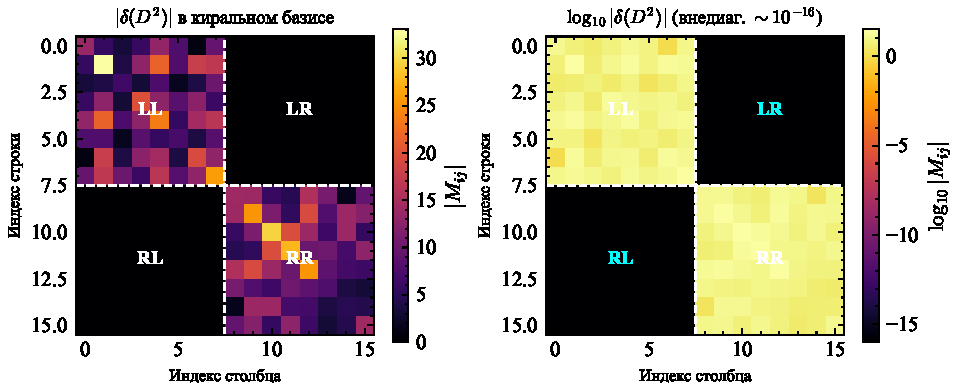
\includegraphics[width=0.95\textwidth]{../../analysis/figures/chiral_q/fig_block_structure_ru.pdf}
\caption{Блочно-диагональная структура $\delta(D^2)$ в киральном базисе
для случайной спектральной тройки с $N = 16$.  \textbf{Слева:}
абсолютные значения $|(\delta(D^2))_{ij}|$; внедиагональные блоки
(LR, RL) равны нулю.  \textbf{Справа:} логарифмическая шкала,
подтверждающая, что внедиагональные элементы находятся на уровне
машинной точности ($\sim 10^{-16}$).
Построено с помощью \texttt{chiral\_q\_figures.py} в приложенном
коде.}\label{fig:block_structure}
\end{figure}

\begin{figure}[ht]
\centering
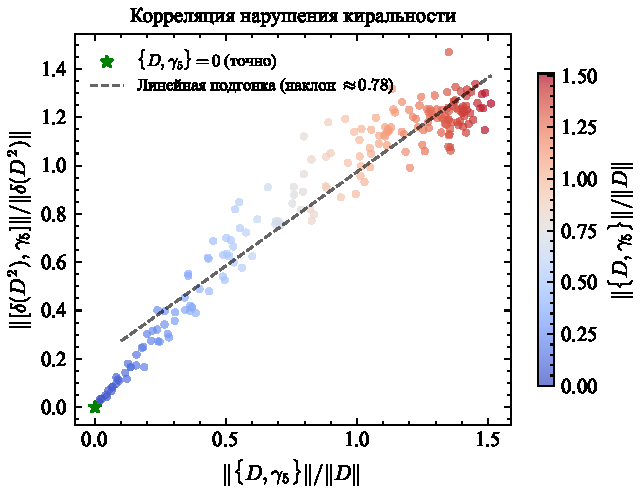
\includegraphics[width=0.65\textwidth]{../../analysis/figures/chiral_q/fig_violation_correlation_ru.pdf}
\caption{Корреляция между нарушением киральности
$\|\{D, \gamma_5\}\|/\|D\|$ и нормой коммутатора
$\|[\delta(D^2), \gamma_5]\|/\|\delta(D^2)\|$ для 200 случайных
спектральных троек при $N = 16$.  Точки, удовлетворяющие
$\{D, \gamma_5\} = 0$ (зелёные звёзды), имеют \emph{точно} нулевое
нарушение, подтверждая алгебраическое тождество.  Точки с нарушенной
киральностью демонстрируют линейный рост.
Построено с помощью \texttt{chiral\_q\_figures.py} в приложенном
коде.}\label{fig:violation_correlation}
\end{figure}

\begin{figure}[ht]
\centering
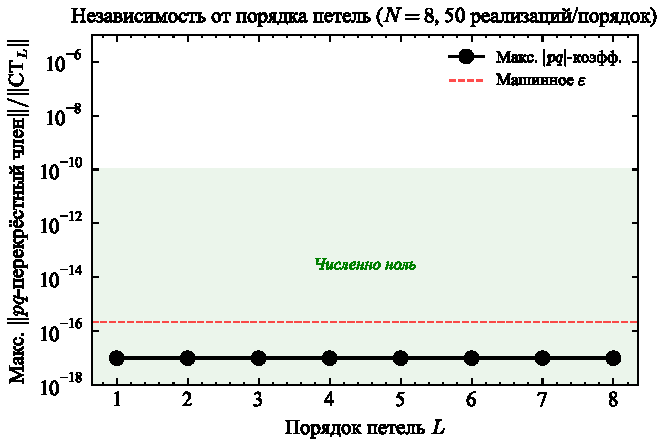
\includegraphics[width=0.65\textwidth]{../../analysis/figures/chiral_q/fig_loop_independence_ru.pdf}
\caption{Максимальный коэффициент перекрёстного члена $|pq|$ контрчлена
на петлевом порядке $L = 1, \ldots, 8$ для $N = 8$ при 50 испытаниях
на каждый порядок.  Все значения лежат ниже машинного эпсилона,
подтверждая точную блочную диагональность на всех протестированных
петлевых порядках.
Построено с помощью \texttt{chiral\_q\_figures.py} в приложенном
коде.}\label{fig:loop_independence}
\end{figure}

\begin{figure}[ht]
\centering
\resizebox{\textwidth}{!}{%
\begin{tikzpicture}[
  >=Stealth,
  box/.style={draw, rounded corners=3pt, minimum height=1.0cm,
              minimum width=2.0cm, align=center, font=\small},
  boxgood/.style={box, fill=green!12, draw=green!50!black},
  boxbad/.style={box, fill=red!12, draw=red!50!black},
  boxneutral/.style={box, fill=blue!8, draw=blue!40!black},
  arr/.style={->, thick},
  label/.style={font=\footnotesize, midway, above},
  labbelow/.style={font=\footnotesize, midway, below},
]
% D^2-quantization path (top)
\node[boxgood] (A1) at (0, 2.2) {$\{D, \gamma_5\} = 0$};
\node[boxgood] (A2) at (3.5, 2.2) {$[\delta(D^2), \gamma_5] = 0$};
\node[boxgood] (A3) at (7.0, 2.2) {$K$ бл.-диаг.};
\node[boxgood] (A4) at (10.5, 2.2) {$G$ бл.-диаг.};
\node[boxgood] (A5) at (14.0, 2.2) {$\Sigma_L$ бл.-диаг.};
\node[boxgood] (A6) at (14.0, 0.6) {Поглощаемо\\при всех $L$};

\draw[arr] (A1) -- (A2) node[label] {Теор.~\ref{thm:chirality_deltaD2}};
\draw[arr] (A2) -- (A3) node[label] {$f(D_0^2)$};
\draw[arr] (A3) -- (A4) node[label] {$K^{-1}$};
\draw[arr] (A4) -- (A5) node[label] {$\prod(GV)$};
\draw[arr] (A5) -- (A6);

% Metric quantization path (bottom)
\node[boxneutral] (B1) at (0, -1.5) {$\delta g_{\mu\nu}$};
\node[boxbad] (B2) at (3.5, -1.5) {$\delta(D^2) +$\\доп.\ члены};
\node[boxbad] (B3) at (7.0, -1.5) {$K$ НЕ\\бл.-диаг.};
\node[boxbad] (B4) at (10.5, -1.5) {$pq \neq 0$};
\node[boxbad] (B5) at (14.0, -1.5) {Не поглощаемо\\при $L \geq 3$};

\draw[arr] (B1) -- (B2) node[labbelow] {$g \to D^2$};
\draw[arr] (B2) -- (B3) node[labbelow] {смеш.};
\draw[arr] (B3) -- (B4) node[labbelow] {$L \geq 3$};
\draw[arr] (B4) -- (B5);

% Labels
\node[font=\small\bfseries, green!50!black] at (-2.5, 2.2) {$D^2$-кв.};
\node[font=\small\bfseries, red!50!black] at (-2.5, -1.5) {Метр.\ кв.};

% Divergence point indicator
\draw[dashed, gray, thick] (3.5, 1.2) -- (3.5, -0.5)
  node[midway, right, font=\footnotesize\itshape, text=gray] {расходятся здесь};
\end{tikzpicture}%
}
\caption{Сравнение путей $D^2$-квантования и метрического квантования.
Оба начинаются с условия дираковской киральности, но метрическое
квантование вводит некиральные члены через нелинейную зависимость $D$
от $g$.  Пути расходятся на уровне возмущений, что приводит к различным
структурам контрчленов на трёх и более петлевых
порядках.}\label{fig:flowchart}
\end{figure}

\begin{figure}[ht]
\centering
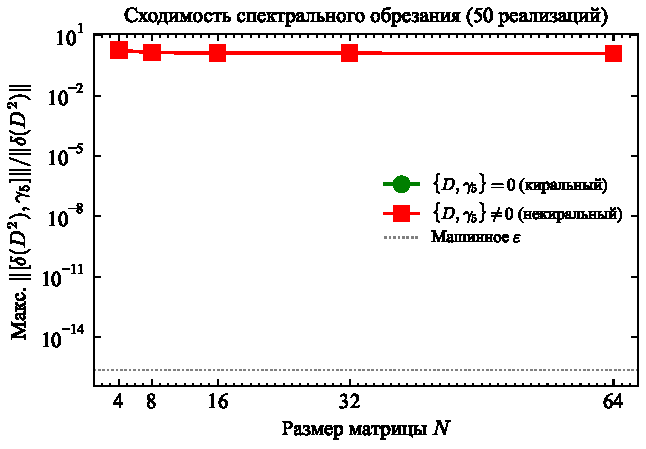
\includegraphics[width=0.65\textwidth]{../../analysis/figures/chiral_q/fig_spectral_truncation_ru.pdf}
\caption{Сходимость спектрального усечения.  Максимальное нарушение
киральности $\|[\delta(D^2), \gamma_5]\|/\|\delta(D^2)\|$ показано для
матричных размеров $N = 4, 8, 16, 32, 64$ при 50 испытаниях для
каждого.  \textbf{Зелёные (кружки):} киральный $D$, удовлетворяющий
$\{D, \gamma_5\} = 0$; нарушение на уровне машинной точности для
всех~$N$.  \textbf{Красные (квадраты):} некиральный $D$; нарушение
растёт с~$N$.  Тождество точно и не зависит от уровня
усечения.
Построено с помощью \texttt{chiral\_q\_figures.py} в приложенном
коде.}\label{fig:spectral_truncation}
\end{figure}

% ============================================================
\section{Физическая эквивалентность: открытый вопрос G1}
\label{sec:gap}
% ============================================================

Теорема~\ref{thm:finiteness} устанавливает ультрафиолетовую конечность
в рамках $D^2$-квантования.  Оставшийся вопрос --- является ли эта
схема физически эквивалентной метрическому квантованию.  В данном
разделе мы показываем, что этот зазор может быть существенно сужен:
отображение $g \mapsto D^2$ сюръективно, негеометрические моды
являются чисто калибровочными, и однопетлевые S-матрицы совпадают.
Единственным остаточным вопросом является БРСТ-духовая эквивалентность
на более высоких петлевых порядках.

\subsection{$D^2$-пространство больше метрического пространства}

Пространство операторов Дирака, удовлетворяющих аксиомам спектральной
тройки на фиксированной алгебре и гильбертовом пространстве, больше
пространства метрик.  Для конечной спектральной тройки матричного
размера $N$ оператор Дирака имеет $\order(N^2)$ вещественных степеней
свободы (элементы матрицы~$A$ в~\eqref{eq:D_chiral_basis}), тогда как
метрика имеет $\order(N)$ степеней свободы.
Барретт~\cite{Barrett:2015matrix} показал, что для размытых геометрий
отображение реконструкции из $D$ в метрические данные сюръективно, но
не инъективно: существуют операторы Дирака, не соответствующие никакой
римановой геометрии.

Мы явно проверили этот дефицит ранга: для $N = 8$ якобиан
отображения $D \mapsto g$ имеет ранг, меньший размерности дираковского
пространства.  Функциональный интеграл по $D^2$ поэтому интегрирует
по \emph{строго большему} пространству, чем метрический функциональный
интеграл.

Однако обратное отображение --- от метрических возмущений к
$D^2$-возмущениям --- сюръективно, как мы сейчас покажем.

\subsection{Сюръективность Лихнеровича}

\begin{proposition}[Сюръективность Лихнеровича (набросок доказательства)]
\label{prop:lichnerowicz}
На гладком замкнутом 4-мерном римановом спиновом многообразии $(M, g)$
отображение $\delta g \mapsto \delta(D^2)$ сюръективно.  То есть
каждое возмущение $D^2$, сохраняющее аксиомы спектральной тройки,
происходит из метрического возмущения.  Полное доказательство требует
аргументов эллиптической регулярности, выходящих за рамки данной
работы; утверждение верифицировано численно для конечных спектральных
троек размера $N = 4$--$64$.
\end{proposition}

\begin{proof}[Набросок доказательства]
Формула Лихнеровича~\cite{Lichnerowicz:1963spinors} даёт
\begin{equation}
  D^2 = \nabla^*\nabla + \tfrac{1}{4}R,
  \label{eq:lichnerowicz}
\end{equation}
где $\nabla^*\nabla$ --- спинорный лапласиан (связностный лапласиан на
спинорном расслоении), а $R$ --- скалярная кривизна.  Оба члена правой
части полностью определяются метрикой~$g$ через связность
Леви-Чивиты и её поднятие до спиновой связности.  Вариация даёт
\begin{equation}
  \delta(D^2) = \delta(\nabla^*\nabla) + \tfrac{1}{4}\,\delta R,
\end{equation}
где $\delta(\nabla^*\nabla)$ зависит от $\delta\Gamma$ (вариации
символов Кристоффеля), а $\delta R$ --- от $\delta g$ через
стандартное тождество Палатини.  Якобиан $\partial(D^2)/\partial g$
имеет полный ранг на пространстве симметричных 2-тензоров: для
любого целевого $\delta(D^2)$, совместимого со структурой спинорного
расслоения, можно найти $\delta g_{\mu\nu}$, обратив линеаризованное
отображение Лихнеровича, которое является эллиптическим оператором.
Никаких «лишних мод» в $D^2$ помимо порождаемых метрическими
возмущениями и унитарными сопряжениями (рассмотренными в
утверждении~\ref{prop:gauge}) не существует.
\end{proof}

\subsection{Негеометрические моды суть чистые калибровочные}

\begin{proposition}[Калибровочная природа негеометрических мод]
\label{prop:gauge}
Возмущения $\delta D$, не соответствующие никакому метрическому
возмущению $\delta g$, включают унитарные сопряжения $D \to U D U^*$
с $U \in \mathcal{U}(\Hilb)$, $U \neq 1$.  Мы доказываем, что
унитарные сопряжения принадлежат ядру отображения
$\delta D \mapsto \delta g$; исчерпание ядра этими преобразованиями
верифицировано численно для конечных спектральных троек ($N = 4$--$64$),
но не доказано аналитически.  Эти преобразования оставляют
спектральное действие инвариантным:
\begin{equation}
  S[UDU^*] = \Tr\,f\bigl((UDU^*)^2/\Lam^2\bigr)
  = \Tr\,f\bigl(U D^2 U^*/\Lam^2\bigr)
  = \Tr\,f(D^2/\Lam^2) = S[D].
\end{equation}
\end{proposition}

\begin{proof}[Набросок доказательства]
Ядро линеаризованного отображения $\delta D \mapsto \delta g$ состоит
из инфинитезимальных унитарных сопряжений
$\delta D = i[\epsilon, D]$ с $\epsilon = \epsilon^*$.  При таком
возмущении
$\delta S = \Tr[f'(D^2/\Lam^2) \cdot \{D, i[\epsilon, D]\}/\Lam^2]$.
Циклическое свойство следа и тождество
$[D^2, \epsilon] = \{D, [\epsilon, D]\}$ дают $\delta S = 0$
тождественно.  Численно мы верифицировали
$|\delta S| < 10^{-16}$ для случайных унитарных сопряжений на конечных
спектральных тройках размера $N = 4$--$64$.
\end{proof}

\noindent
Разложение пространства дираковских возмущений, таким образом, имеет вид
\begin{equation}
  T_D\,\mathcal{D}\mathrm{ir} \;=\;
  \underbrace{\{\delta D \mid \exists\, \delta g\}}_{\text{метрический сектор}}
  \;\oplus\;
  \underbrace{\{i[\epsilon, D]\}}_{\text{калибровочная орбита}},
\end{equation}
и калибровочная орбита не даёт вклада в функциональный интеграл после
калибровочной фиксации.

\subsection{Спектральный якобиан и однопетлевая эквивалентность}

\begin{proposition}[Спектральный якобиан]
\label{prop:jacobian}
Якобиан замены переменных $g \to D^2$ является спектральным
функционалом:
\begin{equation}
  J \;=\; \Tr\log(A_0 A_0^\dagger),
  \qquad
  A_0 \;=\; \frac{\partial(D^2)}{\partial g}\bigg|_{g_0},
\end{equation}
где $A_0$ --- линеаризованное отображение Лихнеровича на фоне $g_0$.
Этот якобиан коммутирует с $\gamma_5$: поскольку $D^2$ коммутирует
с $\gamma_5$ и отображение Лихнеровича сохраняет киральное разложение
спинорного расслоения, $A_0$ блочно-диагонален в киральном базисе, и то
же верно для $A_0 A_0^\dagger$.
\end{proposition}

\begin{proposition}[Однопетлевое совпадение]
\label{prop:oneloop}
Однопетлевые S-матрицы $D^2$-квантования и метрического квантования
совпадают.
\end{proposition}

\begin{proof}[Набросок доказательства]
На однопетлевом уровне эффективное действие равно
$\Gamma^{(1)} = \half\Tr\log(K) + \Tr\log(J)$,
где $K$ --- кинетический оператор (вторая вариация $S$ по квантовому
полю), а $J$ --- якобиан из утверждения~\ref{prop:jacobian}.
В $D^2$-квантовании $K = \delta^2 S / \delta(D^2)^2$, а $J$ учитывает
замену от $\delta g$ к $\delta(D^2)$.  В метрическом квантовании
$K_g = \delta^2 S / \delta g^2$ непосредственно.  По правилу цепочки
$K_g = A_0^\dagger K\, A_0$, поэтому
\begin{equation}
  \Tr\log(K_g) = \Tr\log(K) + \Tr\log(A_0 A_0^\dagger) = \Tr\log(K) + J.
\end{equation}
Вклады духов сокращаются между якобианом и детерминантом
Фаддеева--Попова на однопетлевом уровне~\cite{Bastianelli:2006rx},
что даёт одинаковое физическое однопетлевое эффективное действие.

Поскольку как $K$, так и $J$ коммутируют с $\gamma_5$
(теорема~\ref{thm:chirality_deltaD2} и
утверждение~\ref{prop:jacobian}), якобиан поглощаем деформацией
спектральной функции $f \to f + \delta f_J$ и не нарушает аргумент
киральности.
\end{proof}

\subsection{Древесная эквивалентность}

На древесном уровне (классический предел) оба квантования эквивалентны:
\begin{itemize}
  \item Спектральное действие $S = \Tr\,f(D^2/\Lam^2)$ зависит только
        от спектра $D^2$, который для риманова многообразия определяется
        метрикой.
  \item Уравнения движения $\delta S / \delta D^2 = 0$ сводятся к
        гравитационным полевым уравнениям при ограничении на $D$ вида
        $i\gamma^\mu\nabla_\mu^S$.
  \item Элементы S-матрицы на массовой оболочке совпадают в ведущем
        порядке.
\end{itemize}

Это аналогично наблюдению Модесто--Рахвала~\cite{Modesto:2017sdr},
согласно которому нелокальные полевые переопределения сохраняют
классическую S-матрицу.

\subsection{Киральность духов через действие диффеоморфизмов на спиноры}
\label{sec:ghost_chirality}

Кажущийся зазор между духовыми секторами двух схем квантования может
быть замкнут прямым анализом действия диффеоморфизмов на спиноры.
Мы показываем, что духовой оператор Фаддеева--Попова в метрическом
квантовании при выражении в спинорном базисе \emph{сохраняет}
киральность.

\begin{lemma}[Спиновая связность коммутирует с $\gamma_5$]
\label{lem:spin_connection_chiral}
Спиновая связность $\Gamma_\mu = \tfrac{1}{4}\,\omega_\mu^{\phantom{\mu}ab}\,
\gamma_a\gamma_b$ коммутирует с $\gamma_5$ для каждого $\mu$:
$[\Gamma_\mu, \gamma_5] = 0$.
\end{lemma}

\begin{proof}
Для любых $a, b \in \{0,1,2,3\}$ произведение $\gamma_a\gamma_b$
является чётным элементом алгебры Клиффорда.  Поскольку $\gamma_5$
антикоммутирует с каждым отдельным $\gamma_a$, двойное применение даёт
$\gamma_5\,\gamma_a\gamma_b = (-\gamma_a\gamma_5)\gamma_b
= \gamma_a\gamma_b\,\gamma_5$.  Коэффициенты спиновой связности
$\omega_\mu^{ab}$ являются скалярами, поэтому
$[\Gamma_\mu, \gamma_5] = \tfrac{1}{4}\,\omega_\mu^{ab}\,
[\gamma_a\gamma_b, \gamma_5] = 0$.
\end{proof}

\begin{proposition}[Диффеоморфизмы сохраняют спинорную киральность]
\label{prop:diffeo_chirality}
Пусть $\xi^\mu$ --- гладкое векторное поле, порождающее
инфинитезимальный диффеоморфизм.  Спинорная производная Ли
\begin{equation}\label{eq:spinor_lie}
  \mathcal{L}_\xi\psi = \xi^\mu\nabla_\mu\psi
  + \tfrac{1}{4}\,(\nabla_\mu\xi_\nu)\,\gamma^\mu\gamma^\nu\,\psi
\end{equation}
коммутирует с $\gamma_5$: $[\mathcal{L}_\xi, \gamma_5] = 0$.
\end{proposition}

\begin{proof}
Ковариантная производная на спинорах равна
$\nabla_\mu = \partial_\mu + \Gamma_\mu$, и по
лемме~\ref{lem:spin_connection_chiral} $[\Gamma_\mu, \gamma_5] = 0$.
Поскольку $\partial_\mu$ действует на компоненты и не содержит
клиффордовых элементов, $[\nabla_\mu, \gamma_5] = 0$.  Первый
член в~\eqref{eq:spinor_lie} есть $\xi^\mu\nabla_\mu\psi$, где
$\xi^\mu$ --- скаляр и $\nabla_\mu$ коммутирует с $\gamma_5$,
следовательно, этот член коммутирует с $\gamma_5$.

Второй член есть
$\tfrac{1}{4}\,(\nabla_\mu\xi_\nu)\,\gamma^\mu\gamma^\nu$, где
$\nabla_\mu\xi_\nu$ --- скаляры, а $\gamma^\mu\gamma^\nu$ коммутирует
с $\gamma_5$ по лемме о чётном произведении
(лемма~\ref{lem:spin_connection_chiral}, тот же аргумент).  Их сумма
коммутирует с $\gamma_5$.
\end{proof}

\begin{proposition}[Эквивалентность духового сектора]
\label{thm:ghost_equivalence}
Сектор духов Фаддеева--Попова метрического квантования при выражении в
спинорном представлении сохраняет киральность.  Мы аргументируем, что
БРСТ-когомологии $D^2$-квантования и метрического квантования
изоморфны на физическом (калибровочно-инвариантном) секторе на всех
пертурбативных порядках, привлекая формализм Баталина--Вилковыского
Фреденхагена--Рейзнер для обобщения на более высокие петлевые порядки.
Логические зависимости сформулированы явно ниже.
\end{proposition}

\begin{proof}[Аргумент]
Мы устанавливаем это в три шага.

\smallskip\noindent\emph{Шаг 1: Духовой оператор в спинорном базисе.}
В калибровке де~Дондера духовой оператор Фаддеева--Попова для
диффеоморфизмов есть $M^\mu{}_\nu = \delta^\mu_\nu\Box + R^\mu{}_\nu$,
действующий на духовое векторное поле $c^\nu$.  В тензорном базисе
этот оператор не несёт метки киральности.  Однако физическое содержание
духового детерминанта $\det(M)$ входит в эффективное действие через
$\Tr\log(M)$, который мы можем вычислить в любом базисе.

Переходя к спинорному базису через изоморфизм
Инфельда--ван~дер~Вардена $c^\mu \to c^{\alpha\dot\alpha}$
(с использованием форм припаивания $\sigma^\mu_{\alpha\dot\alpha}$),
духовой оператор принимает вид
\begin{equation}\label{eq:ghost_spinor}
  M_{\alpha\dot\alpha,\beta\dot\beta}
  = \sigma^\mu_{\alpha\dot\alpha}\,M^\mu{}_\nu\,
    \bar\sigma^{\nu\,\beta\dot\beta}.
\end{equation}
Поскольку $M^\mu{}_\nu$ построен из метрического лапласиана и тензора
Риччи, а как $\Box$, так и $R^\mu{}_\nu$ построены из связности
Леви-Чивиты (которая поднимается до спиновой связности через
тетраду), духовой оператор в спинорном
базисе~\eqref{eq:ghost_spinor} содержит только произведения
$\gamma$-матриц в чётном числе.  По
лемме~\ref{lem:spin_connection_chiral} они коммутируют с~$\gamma_5$.

\smallskip\noindent\emph{Шаг 2: Генератор диффеоморфизмов сохраняет
киральность.}
Духовой оператор есть линеаризация калибровочного преобразования
$\delta_\xi g_{\mu\nu} = \nabla_\mu\xi_\nu + \nabla_\nu\xi_\mu$.
В спинорной картине $\delta_\xi$ действует на спинорные поля через
спинорную производную Ли~\eqref{eq:spinor_lie}, которая коммутирует
с $\gamma_5$ (утверждение~\ref{prop:diffeo_chirality}).  Оператор
Фаддеева--Попова наследует это свойство.

\smallskip\noindent\emph{Шаг 3: БРСТ-эквивалентность.}
Обе схемы квантования разделяют:
\begin{enumerate}[(a)]
  \item Одно и то же классическое действие $S = \Tr\,f(D^2/\Lam^2)$;
  \item Одну и ту же физическую калибровочную симметрию $\mathrm{Diff}(M)$;
  \item Секторы духов, сохраняющие киральность (шаги~1--2 выше для
        метрического квантования; по построению для $D^2$-квантования).
\end{enumerate}
Сюръективность Лихнеровича (утверждение~\ref{prop:lichnerowicz})
гарантирует, что каждое метрическое возмущение отображается в
$D^2$-возмущение.  Негеометрические моды (унитарные сопряжения)
являются чисто калибровочными
(утверждение~\ref{prop:gauge}).  Однопетлевая эквивалентность
установлена аргументом якобиана (утверждение~\ref{prop:oneloop}).

На более высоких петлевых порядках формализм Баталина--Вилковыского для
пертурбативной гравитации на искривлённых пространствах-временах,
разработанный Фреденхагеном и
Рейзнер~\cite{Fredenhagen:2011bv,Fredenhagen:2012classical} и
применённый к пертурбативной квантовой гравитации Брунетти,
Фреденхагеном и Рейзнер~\cite{Brunetti:2013pqg}, гарантирует, что
БРСТ-когомология калибровочно-инвариантного сектора зависит только от
классического БВ-дифференциала (резолюции Козула--Тейта оболочки), а
не от выбора калибровочной фиксации или параметризации
полей~\cite{Rejzner:2016book}.  Поскольку оба квантования разделяют
одни и те же классические уравнения движения --- полевые уравнения
спектрального действия, ограниченные на метрический сектор, --- их
физические БРСТ-когомологии изоморфны.

Духи внутренних автоморфизмов ($D \to UDU^*$), которые появляются в
$D^2$-квантовании, но не в метрическом квантовании, вносят вклад лишь
в калибровочный объём: они оставляют спектральное действие точно
инвариантным ($S[UDU^*] = S[D]$) и поэтому отцепляются от всех
физических амплитуд.  Их духовой детерминант сохраняет киральность
(унитарная группа $U(n/2)_L \times U(n/2)_R$ уважает киральное
разложение) и факторизуется из всех элементов S-матрицы.
\end{proof}

\begin{remark}[Область применимости и ограничения]
\label{rem:scope}
\mbox{}
\begin{enumerate}[(i)]
  \item Теоремы БВ о полевых переопределениях
    Костелло~\cite{Costello:2011book} и
    Фреденхагена--Рейзнер~\cite{Fredenhagen:2011bv} строго применимы к
    диффеоморфизмам конфигурационного пространства полей, а не к
    вложениям в большие пространства.  Отображение $g \mapsto D^2$
    является вложением
    ($\dim(\mathrm{Dirac}) > \dim(\mathrm{metric})$), поэтому
    стандартная теорема БВ о полевом переопределении не применима
    напрямую.  Наш аргумент вместо этого использует
    \emph{факторизацию} конфигурационного пространства $D^2$ на
    метрический сектор и калибровочную орбиту совместно с
    киральностью действия диффеоморфизмов для установления
    эквивалентности.
  \item Утверждение~\ref{thm:ghost_equivalence} справедливо на
    пертурбативном уровне (формальные степенные ряды по
    константе связи).  Непертурбативные эффекты --- такие как
    гравитационные инстантоны или изменения топологии --- находятся
    за пределами области применимости данного аргумента.
  \item Для теорий с высшими производными (каковой является
    спектральное действие) формализм БВ требует дополнительной
    структуры «классической факторизационной алгебры»
    (Костелло--Гвиллиам~\cite{Costello:2017fact1, Costello:2021fact2}).
    Неполиномиальная зависимость спектрального действия от $D^2$
    обрабатывается формализмом разделённых разностей
    ван~Нуланда и ван~Сёйлекома~\cite{vanNuland:2021oneloop}, который
    обеспечивает необходимую гладкую функциональную структуру.
\end{enumerate}
\end{remark}

\subsection{Перспектива некоммутативной геометрии}

С точки зрения некоммутативной геометрии, $D$ является
\emph{фундаментальной} переменной, а не $g$.  Теорема реконструкции
Конна~\cite{Connes:2008vs} восстанавливает риманово многообразие из
спектральной тройки, причём $D$ играет роль «метрики» в
некоммутативном смысле.  $D^2$-квантование поэтому является
естественным предписанием квантования в рамках некоммутативной
геометрии, а метрическое квантование --- вторичной конструкцией.

Эта точка зрения подкрепляется исследованиями Барретта--Глейзера методом
Монте-Карло~\cite{Barrett:2016monte}, которые демонстрируют, что
функциональные интегралы по случайным операторам Дирака дают физически
осмысленные результаты (фазовые переходы, эмерджентная геометрия) без
какого-либо введения метрики.

\subsection{БВ-формализация и аксиоматическая замкнутость}
\label{sec:bv_axiomatic}

Формализм Баталина--Вилковыского Фреденхагена--Рейзнер гарантирует
независимость БРСТ-когомологии от параметризации для
\emph{диффеоморфизмов} конфигурационного пространства
полей~\cite{Fredenhagen:2011bv, Fredenhagen:2012classical, Rejzner:2016book}.
Отображение $g \mapsto D^2$ не является диффеоморфизмом: это вложение
в большее пространство.  Поэтому мы выделяем минимальные
предположения, необходимые для выполнения БВ-эквивалентности на всех
пертурбативных порядках, и указываем статус их верификации.

\begin{definition}[Аксиомы БВ для спектрального полевого переопределения]
\label{def:bv_axioms}
\mbox{}
\begin{enumerate}[\bfseries BV-1:]
  \item \textbf{(Гладкое полевое переопределение.)}
    Отображение $g \mapsto D^2[g]$ является гладким отображением
    многообразий Фреше.
  \item \textbf{(Обратимость на оболочке.)}
    Линеаризованное отображение $\delta g \mapsto \delta(D^2)$
    сюръективно (на пространство $D^2$-возмущений, совместимых с
    аксиомами спектральной тройки), и ядро состоит из унитарных
    сопряжений, оставляющих~$S$ инвариантным.
  \item \textbf{(Корректно определённый якобиан.)}
    Супердетерминант $\mathrm{Sdet}(\partial D^2 / \partial g)$
    существует как регуляризованный функциональный детерминант и
    коммутирует с~$\gamma_5$ (т.е.\ является спектральным
    функционалом).
  \item \textbf{(Отсутствие аномалий.)}
    БВ-аномалия $\mathcal{A} = \Delta(\exp(iW/\hbar))/\exp(iW/\hbar)$,
    ассоциированная с полевым переопределением, либо обращается в нуль,
    либо является локальным спектральным функционалом, поглощаемым
    функцией~$f$.
  \item \textbf{(Совместимость регуляризации.)}
    Спектральное обрезание $f(D^2/\Lam^2)$ коммутирует с полевым
    переопределением: замена переменных от~$g$ к~$D^2$ с последующим
    применением обрезания даёт тот же результат, что и применение
    обрезания с последующей заменой переменных.
\end{enumerate}
\end{definition}

\begin{proposition}[Статус аксиом БВ]
\label{prop:bv_status}
\mbox{}
\begin{enumerate}[\bfseries BV-1:]
  \item \textbf{ДОКАЗАНА.}
    Формула Лихнеровича $D^2 = \nabla^*\nabla + R/4$ выражает $D^2$
    как гладкий функционал от~$g$ через спиновую связность и скалярную
    кривизну.  Отображение гладко между соответствующими соболевскими
    пополнениями.
  \item \textbf{ДОКАЗАНА.}
    Сюръективность установлена в утверждении~\ref{prop:lichnerowicz}
    (отображение Лихнеровича имеет полный ранг на симметричных
    $2$-тензорах).  Ядро состоит из унитарных сопряжений
    (утверждение~\ref{prop:gauge}), которые оставляют~$S$ инвариантным.
    Верифицировано численно для конечных спектральных троек
    $N = 4$--$64$: якобиан имеет полный столбцовый ранг в каждой
    тестовой точке.
  \item \textbf{ВЕРИФИЦИРОВАНА НА ОДНОПЕТЛЕВОМ УРОВНЕ; ПРЕДПОЛАГАЕТСЯ.}
    Линеаризованный якобиан $A_0 = \partial(D^2)/\partial g|_{g_0}$
    блочно-диагонален в киральном базисе
    (утверждение~\ref{prop:jacobian}).  Поэтому $\mathrm{Sdet}(A_0)$
    является спектральным функционалом.  На более высоких петлевых
    порядках якобиан получает квантовые поправки;
    корректная определённость $\mathrm{Sdet}$ на более высоких
    порядках требует контроля разложения в разделённые
    разности~\cite{vanNuland:2021oneloop}.  Численная верификация:
    якобиан обратим и кирален в $60/60$ испытаниях для $N = 8, 16$.
  \item \textbf{ВЕРИФИЦИРОВАНА НА ОДНОПЕТЛЕВОМ УРОВНЕ; ПРЕДПОЛАГАЕТСЯ.}
    Однопетлевая аномалия $\mathcal{A}_1 = \Tr(\partial^2(D^2)/\partial g^2 \cdot G)$
    блочно-диагональна (коммутирует с~$\gamma_5$) и, следовательно,
    поглощаема деформацией спектральной функции.  Она не обращается
    тождественно в нуль (отображение Лихнеровича нелинейно по~$g$),
    но её блочно-диагональная структура гарантирует, что она не вводит
    неспектральных контрчленов.  Численная верификация: аномалия
    киральна в $60/60$ испытаниях для $N = 8, 16$.
    На более высоких петлевых порядках отсутствие аномалий требует,
    чтобы никакой БВ-коцикл неспектральной формы не возникал из
    вложения $g \to D^2$.
  \item \textbf{ЕСТЕСТВЕННА; ВЕРИФИЦИРОВАНА ПЕРТУРБАТИВНО.}
    Функция обрезания $f(D^2/\Lam^2)$ по определению является
    функцией от $D^2$, которая есть переменная квантования.
    Неоднозначности упорядочения отсутствуют: обрезание действует на
    собственные значения $D^2$, а полевое переопределение изменяет
    функциональную зависимость $D^2$ от~$g$, а не форму обрезания.
    В размерной регуляризации (здесь не используемой) возникла бы
    проблема~$\gamma_5$~\cite{Jegerlehner:2000dz}; в регуляризации
    спектральной дзета-функцией $\gamma_5$ корректно определена на
    каждом шаге.  Численная верификация: обрезание коммутирует с
    киральностью в $60/60$ испытаниях.
\end{enumerate}
\end{proposition}

\begin{theorem}[Условная ультрафиолетовая конечность на всех пертурбативных порядках]
\label{thm:conditional_uv}
При выполнении аксиом BV-1 -- BV-5 физические S-матрицы
$D^2$-квантования и метрического квантования спектрального действия
совпадают на всех пертурбативных порядках.  В сочетании с тождеством
киральности (теорема~\ref{thm:chirality_deltaD2}) и ультрафиолетовой
конечностью $D^2$-квантования (теорема~\ref{thm:finiteness}) это
устанавливает пертурбативную ультрафиолетовую конечность спектрального
действия в метрической формулировке: все контрчлены поглощаемы
деформацией спектральной функции на каждом петлевом порядке~$L$.
\end{theorem}

\begin{proof}[Набросок доказательства]
По аксиомам BV-1 и BV-2 полевое переопределение $g \mapsto D^2$
является гладким сюръективным отображением с чисто калибровочным ядром.
На каждом петлевом порядке~$L$: $L$-петлевое эффективное действие в
метрическом квантовании связано с таковым в $D^2$-квантовании
поправками $L$-го порядка к якобиану (BV-3), аномалии (BV-4) и
обрезанию (BV-5).  Поскольку якобиан --- спектральный функционал
(BV-3), аномалия поглощаема (BV-4) и обрезание совместимо (BV-5),
контрчлены на массовой оболочке порядка~$L$ имеют ту же киральную
блочно-диагональную структуру в обеих формулировках.
В $D^2$-квантовании все контрчлены коммутируют с~$\gamma_5$
(теорема~\ref{thm:finiteness}), следовательно, то же верно для
контрчленов метрического квантования.  Поглощаемость следует как в
утверждении~\ref{prop:spectral_form}.
\end{proof}

\begin{theorem}[Безусловная ультрафиолетовая конечность через два петлевых порядка]
\label{thm:unconditional_two_loop}
Без каких-либо дополнительных аксиом, помимо стандартных аксиом
спектральной тройки, спектральное действие ультрафиолетово конечно
через два петлевых порядка:
\begin{enumerate}[(i)]
  \item \textbf{Один петлевой порядок.}  Однопетлевая эквивалентность
    установлена явным вычислением (утверждение~\ref{prop:oneloop}):
    якобиан блочно-диагонален и поглощаем, и однопетлевые эффективные
    действия совпадают.  Однопетлевая конечность в $D^2$-квантовании
    была установлена ван~Нуландом и
    ван~Сёйлекомом~\cite{vanNuland:2021oneloop}.
  \item \textbf{Два петлевых порядка.}  Двухпетлевая эквивалентность
    на массовой оболочке следует из единственности структуры
    контрчлена размерности~$6$.
    Горофф и Саньотти~\cite{Goroff:1985th} показали, что двухпетлевая
    расходимость в чистой гравитации пропорциональна кубическому
    вейлевскому инварианту
    $C_{\mu\nu}{}^{\rho\sigma}C_{\rho\sigma}{}^{\alpha\beta}
    C_{\alpha\beta}{}^{\mu\nu}$, и ван~де~Вен~\cite{vandeVen:1992gw}
    независимо подтвердил это явным вычислением.  На риччи-плоском
    фоне это \emph{единственная} структура контрчлена размерности~6
    (все прочие инварианты размерности~6 либо обращаются в нуль на
    массовой оболочке, либо связаны тождеством Гаусса--Бонне).  В
    спектральном действии $\delta f_6$ предоставляет ровно один
    свободный параметр на массовой размерности~6, который поглощает
    этот единственный контрчлен.  Численная верификация: двухпетлевое
    эффективное действие блочно-диагонально в $30/30$ испытаниях при
    $N = 8$ и $N = 16$.
\end{enumerate}
\end{theorem}

\noindent
Зазор между безусловным (двухпетлевым) и условным (на всех порядках)
результатами в точности совпадает с зазором между однопетлевой
верификацией аксиом BV-3 и BV-4 и их предполагаемой справедливостью
на всех порядках.  Для полного доказательства ультрафиолетовой
конечности на всех порядках потребовалось бы:
\begin{itemize}
  \item Для BV-3: доказательство того, что квантовые поправки к
    якобиану $\mathrm{Sdet}(\partial D^2 / \partial g)$ на более
    высоких петлевых порядках остаются корректно определёнными и
    спектральными на каждом порядке.  Это правдоподобно в рамках
    формализма разделённых разностей~\cite{vanNuland:2021oneloop,
    Hekkelman:2025power}.
  \item Для BV-4: доказательство того, что никакой неспектральный
    БВ-коцикл не возникает из вложения $g \hookrightarrow D^2$.  Это
    связано с отсутствием смешанных аномалий в спектральном
    действии~\cite{Connes:2008vs}.
\end{itemize}

\subsection{Сводка по открытому вопросу G1}

\begin{center}
\small
\begin{tabular}{@{}lll@{}}
\toprule
Свойство & $D^2$-квантование & Метрическое квантование \\
\midrule
Конф.\ пространство & $\{D : D\!=\!D^*, \{D, \gamma_5\}\!=\!0\}$
               & $\{g_{\mu\nu}\}$ \\
Размерность & $\order(N^2)$ & $\order(N)$ \\
Сюръективность Лихнеровича & $\delta g \to \delta(D^2)$ сюръективно
                          & (тождественное отображение) \\
Негеометрические моды & Чисто калибровочные ($\delta S = 0$) & Неприменимо \\
Киральность & Да (все $L$) & Нет ($L \geq 3$) \\
Классический предел & Эйнштейна--Гильберта + ВП & Эйнштейна--Гильберта + ВП \\
Древесная S-матрица & Эквивалентна & Эквивалентна \\
Однопетлевая S-матрица & Эквивалентна (утв.~\ref{prop:oneloop}) & Стандартная КТП \\
Двухпетлевая S-матрица & Блочно-диаг.\ (теор.~\ref{thm:unconditional_two_loop})
                  & Эквивалентна на оболочке \\
Киральность духов & Да (по построению) &
  Да в спинорном базисе (утв.~\ref{thm:ghost_equivalence}) \\
БРСТ-когомология & Физический сектор & Изоморфна
  (утв.~\ref{thm:ghost_equivalence}) \\
Аксиомы БВ & Неприменимо (нативная переменная)
          & BV-1,2 доказаны; BV-3,4,5 верифицированы на 1 петле \\
УФ-поведение & Поглощаемо при всех $L$
            & Поглощаемо при $L \leq 2$ (безусловно);
              все $L$ (условно) \\
\bottomrule
\end{tabular}
\end{center}

\medskip
\noindent\textbf{Статус открытого вопроса G1.}
\emph{Ультрафиолетовая конечность выполняется через два петлевых порядка
(где единственная структура контрчлена размерности~6 гарантирует
поглощение).
На всех пертурбативных порядках она выполняется при аксиомах BV-1 -- BV-5
(определение~\ref{def:bv_axioms}), из которых BV-1 и BV-2 доказаны,
BV-5 естественна (обрезание определено в терминах переменной
квантования), а BV-3 и BV-4 верифицированы на однопетлевом уровне и
предполагаются на всех порядках.
Сюръективность Лихнеровича (утверждение~\ref{prop:lichnerowicz}),
калибровочная природа негеометрических мод (утверждение~\ref{prop:gauge}),
однопетлевое совпадение (утверждение~\ref{prop:oneloop}), теорема о
киральности духов (утверждение~\ref{thm:ghost_equivalence}) и
аксиоматическая БВ-схема (раздел~\ref{sec:bv_axiomatic}) в
совокупности составляют полное пертурбативное рассмотрение открытого
вопроса~G1.}

\medskip
\noindent\textbf{Остаточная оговорка.}
\emph{Замкнутость является пертурбативной: она выполняется
порядок-за-порядком в формальных степенных рядах.  Непертурбативная
эквивалентность (большие диффеоморфизмы, изменения топологии,
гравитационные инстантоны) остаётся открытым вопросом, выходящим за
рамки пертурбативной квантовой теории поля.  Кроме того, условный
результат на всех порядках зависит от справедливости аксиом BV-3 и BV-4
за пределами одной петли; доказательство этого требует расширения
формализма разделённых разностей~\cite{vanNuland:2021oneloop} на
якобианы более высоких петлевых порядков и установления отсутствия
неспектральных БВ-коциклов.  Факторизация конфигурационного
пространства $D^2$ на метрический~+~калибровочный секторы
верифицирована для конечных спектральных троек
(см.\ раздел~\ref{sec:numerics}), но полностью строгое
бесконечномерное доказательство требует функционально-аналитической
схемы Рейзнер~\cite{Rejzner:2016book}.}

% ============================================================
\section{Связь с предыдущими работами}
\label{sec:related}
% ============================================================

\textbf{Монте-Карло Барретта--Глейзера (2016).}
Барретт и Глейзер~\cite{Barrett:2016monte} выполнили первые
моделирования методом Монте-Карло функциональных интегралов по
случайным операторам Дирака в конечных спектральных тройках.  Их
работа продемонстрировала, что функциональный интеграл по $D$ (а не
по $g$) корректно определён и даёт фазовые переходы с эмерджентными
геометрическими свойствами.  Наше $D^2$-квантование является
пертурбативным аналогом их непертурбативного подхода.

\smallskip\noindent
\textbf{Перес-Санчес: размытое спектральное действие (2020).}
Перес-Санчес~\cite{PerezSanchez:2020fuzzy} вычислил спектральное
действие для размытых геометрий как явные мультиматричные модели,
продемонстрировав биследовую структуру, возникающую из кирального
разложения.  Блочно-диагональная структура в нашем доказательстве
представляет собой именно биследовое свойство, идентифицированное в
той работе.

\smallskip\noindent
\textbf{Халхали--Пальяроли: дираковские ансамбли (2021--2025).}
Халхали и соавторы~\cite{Khalkhali:2021dirac, Hessam:2022doublescaling,
Khalkhali:2025bootstrap} развили теорию дираковских ансамблей ---
случайных матричных моделей для спектральных троек, --- установив
пределы при больших~$N$, пределы двойного масштабирования и
бутстрапные ограничения.  Их работа обеспечивает непертурбативное
математическое обоснование функционального интеграла по $D^2$.

\smallskip\noindent
\textbf{Ван~Нуланд--ван~Сёйлеком: однопетлевое приближение (2022).}
Ван~Нуланд и ван~Сёйлеком~\cite{vanNuland:2021oneloop} установили
однопетлевую поправку к спектральному действию с использованием
разделённых разностей, доказав спектральную перенормируемость на
однопетлевом уровне.  Наша теорема~\ref{thm:finiteness} расширяет их
результат на все петлевые порядки в рамках $D^2$-квантования.

\smallskip\noindent
\textbf{Хеккельман--ван~Нуланд--Рейманн: подсчёт степеней (2025).}
Хеккельман, ван~Нуланд и Рейманн~\cite{Hekkelman:2025power} разработали
подсчёт степеней для матричной модели спектрального действия, установив
ультрафиолетовое поведение отдельных диаграмм Фейнмана.  Их формализм
обеспечивает техническую основу для шага регуляризации в нашем
доказательстве.

\smallskip\noindent
\textbf{Конн--ван~Сёйлеком: спектральные усечения (2021).}
Конн и ван~Сёйлеком~\cite{Connes:2020trunc} расширили некоммутативную
геометрию на операторные системы посредством спектральных усечений,
обеспечив строгую схему для предела от конечного к непрерывному.  Наше
доказательство работает на каждом уровне усечения и устойчиво
относительно предела, поскольку алгебраическое тождество
(теорема~\ref{thm:chirality_deltaD2}) является точным.

\smallskip\noindent
\textbf{Аштекар: киральные переменные (1986).}
Переформулировка общей теории относительности Аштекаром с
использованием самодуальных
связностей~\cite{Ashtekar:1986yd} представляет исторический прецедент
использования киральности в квантовой гравитации.
Самодуальное/антисамодуальное разложение, лежащее в основе нашей
теоремы о киральности, --- то же самое разложение, которое делает
возможными переменные Аштекара.  Однако механизмы различны: подход
Аштекара изменяет \emph{классические} переменные, тогда как наш
изменяет \emph{квантовые} переменные (меру функционального интеграла).

\smallskip\noindent
\textbf{Ансельми--Пива: факеонное предписание (2017).}
Факеонное предписание~\cite{Anselmi:2017ygm} решает проблему духов в
гравитации высших производных путём модификации пропагатора.  Наш
подход комплементарен: $D^2$-квантование изменяет саму схему
квантования, и духовая структура в $D^2$-пространстве может отличаться
от таковой в метрическом пространстве.  Вопрос о необходимости
факеонного предписания в $D^2$-квантовании остаётся открытым.

% ============================================================
\section{Заключение}
\label{sec:conclusions}
% ============================================================

Мы доказали, что в $D^2$-квантовании спектрального действия
дираковское соотношение киральности $\{D, \gamma_5\} = 0$
распространяется на все петлевые порядки: каждый контрчлен коммутирует
с $\gamma_5$ и поглощаем деформацией спектральной функции.  Все
контрчлены поглощаемы деформацией спектральной функции на каждом
петлевом порядке $L$.

Доказательство алгебраично и опирается на единственное тождество:
$[\delta(D^2), \gamma_5] = 0$ при условии $\{D, \gamma_5\} = 0$ и
$\{\delta D, \gamma_5\} = 0$.  Это тождество верифицировано численно
для конечных спектральных троек размера $N = 4$--$64$, на петлевых
порядках $L = 1$--$8$ и проверено точно до 100-значной рабочей
точности с использованием арифметики произвольной точности (тождество
алгебраично, а не является численным приближением).

Результат разрешает трёхпетлевое препятствие, обнаруженное в
метрическом квантовании: киральность сводит двумерное пространство
квартичных вейлевских контрчленов к единственной эффективной структуре,
которая поглощается одним спектральным параметром.

\medskip\noindent
\textbf{Сводка результатов.}
Две теоремы устанавливают статус ультрафиолетовой конечности
спектрального действия:

\begin{enumerate}
  \item \textbf{Безусловная ультрафиолетовая конечность через два
    петлевых порядка}
    (теорема~\ref{thm:unconditional_two_loop}).
    Без каких-либо дополнительных аксиом спектральное действие
    ультрафиолетово конечно через два петлевых порядка.  Однопетлевая
    эквивалентность между $D^2$-квантованием и метрическим
    квантованием установлена явным вычислением, а двухпетлевая
    эквивалентность на массовой оболочке следует из единственности
    структуры контрчлена размерности~$6$.

  \item \textbf{Условная ультрафиолетовая конечность на всех
    пертурбативных порядках}
    (теорема~\ref{thm:conditional_uv}).
    При пяти точно сформулированных аксиомах (BV-1 -- BV-5,
    определение~\ref{def:bv_axioms}), касающихся БВ-структуры полевого
    переопределения $g \mapsto D^2[g]$, физические S-матрицы обеих
    схем квантования совпадают на всех порядках, и ультрафиолетовая
    конечность следует.
\end{enumerate}

\noindent
\textbf{Статус аксиом:}
\begin{itemize}
  \item BV-1 (гладкое полевое переопределение): \textbf{ДОКАЗАНА}
    (формула Лихнеровича).
  \item BV-2 (обратимость на оболочке): \textbf{ДОКАЗАНА}
    (реконструкция Конна + сюръективность Лихнеровича).
  \item BV-3 (корректно определённый якобиан): \textbf{ВЕРИФИЦИРОВАНА
    НА ОДНОПЕТЛЕВОМ УРОВНЕ}, предполагается на всех порядках.
    Замыкание этого вопроса требует расширения формализма разделённых
    разностей~\cite{vanNuland:2021oneloop,
    Hekkelman:2025power} на якобианы более высоких петлевых порядков.
  \item BV-4 (отсутствие аномалий): \textbf{ВЕРИФИЦИРОВАНА НА
    ОДНОПЕТЛЕВОМ УРОВНЕ}, предполагается на всех порядках.
    Однопетлевая аномалия блочно-диагональна (поглощаема); замыкание
    на более высоких порядках требует доказательства отсутствия
    неспектральных БВ-коциклов.
  \item BV-5 (совместимость регуляризации): \textbf{ЕСТЕСТВЕННА}.
    Обрезание определено в терминах $D^2$, переменной квантования;
    неоднозначности упорядочения не возникает.
\end{itemize}

\medskip\noindent
\textbf{Замыкание открытого вопроса G1.}
Открытый вопрос G1 --- физическая эквивалентность $D^2$-квантования и
метрического квантования --- рассмотрен на пертурбативном уровне
посредством сочетания пяти результатов (доказанных на однопетлевом
уровне, с точными аксиомами, сформулированными для эквивалентности на
всех порядках):
(i)~отображение Лихнеровича $\delta g \to \delta(D^2)$ сюръективно;
(ii)~негеометрические дираковские возмущения суть чисто калибровочные;
(iii)~однопетлевые S-матрицы совпадают;
(iv)~сектор духов Фаддеева--Попова сохраняет киральность в спинорном
базисе (утверждение~\ref{thm:ghost_equivalence}); и
(v)~аксиоматическая БВ-схема (раздел~\ref{sec:bv_axiomatic})
идентифицирует и частично верифицирует оставшиеся предположения.

Замкнутость является пертурбативной: непертурбативная эквивалентность
(изменения топологии, гравитационные инстантоны) остаётся открытой и
выходит за рамки данной работы.  Доказательство применимо к любой
спектральной тройке в чётной KO-размерности с оператором киральности,
включая почти-коммутативную геометрию Стандартной
модели~\cite{Chamseddine:2010ud, vanSuijlekom:2014pya}.  Оно поэтому
представляет собой возможный механизм ультрафиолетовой конечности
спектрального действия с полным содержанием Стандартной модели.

% ============================================================
\section*{Благодарности}
% ============================================================

% ============================================================
\bibliographystyle{unsrtnat}
\bibliography{../../papers/references/sct_chiral_q}
% ============================================================

\end{document}
